\documentclass[presentation]{beamer}

\usepackage{appendixnumberbeamer}
\usepackage{amsmath}
\date{3rd March 2017}
\usetheme{firedrake}

\author{Lawrence Mitchell\inst{1}}
\institute{\inst{1}Departments of Computing and Mathematics, Imperial College London}
\title{z-layers, oh noes}

\graphicspath{{./\jobname.figures/}}

\newcommand{\arxivlink}[2]{%
  \href{http://www.arxiv.org/abs/#1}%
  {{\small\texttt{arXiv:\,#1\,[#2]}}}%
}
\usepackage{minted}

\begin{document}

\maketitle

\begin{frame}[plain]
  \begin{columns}
    \begin{column}{\textwidth}
      \only<1>{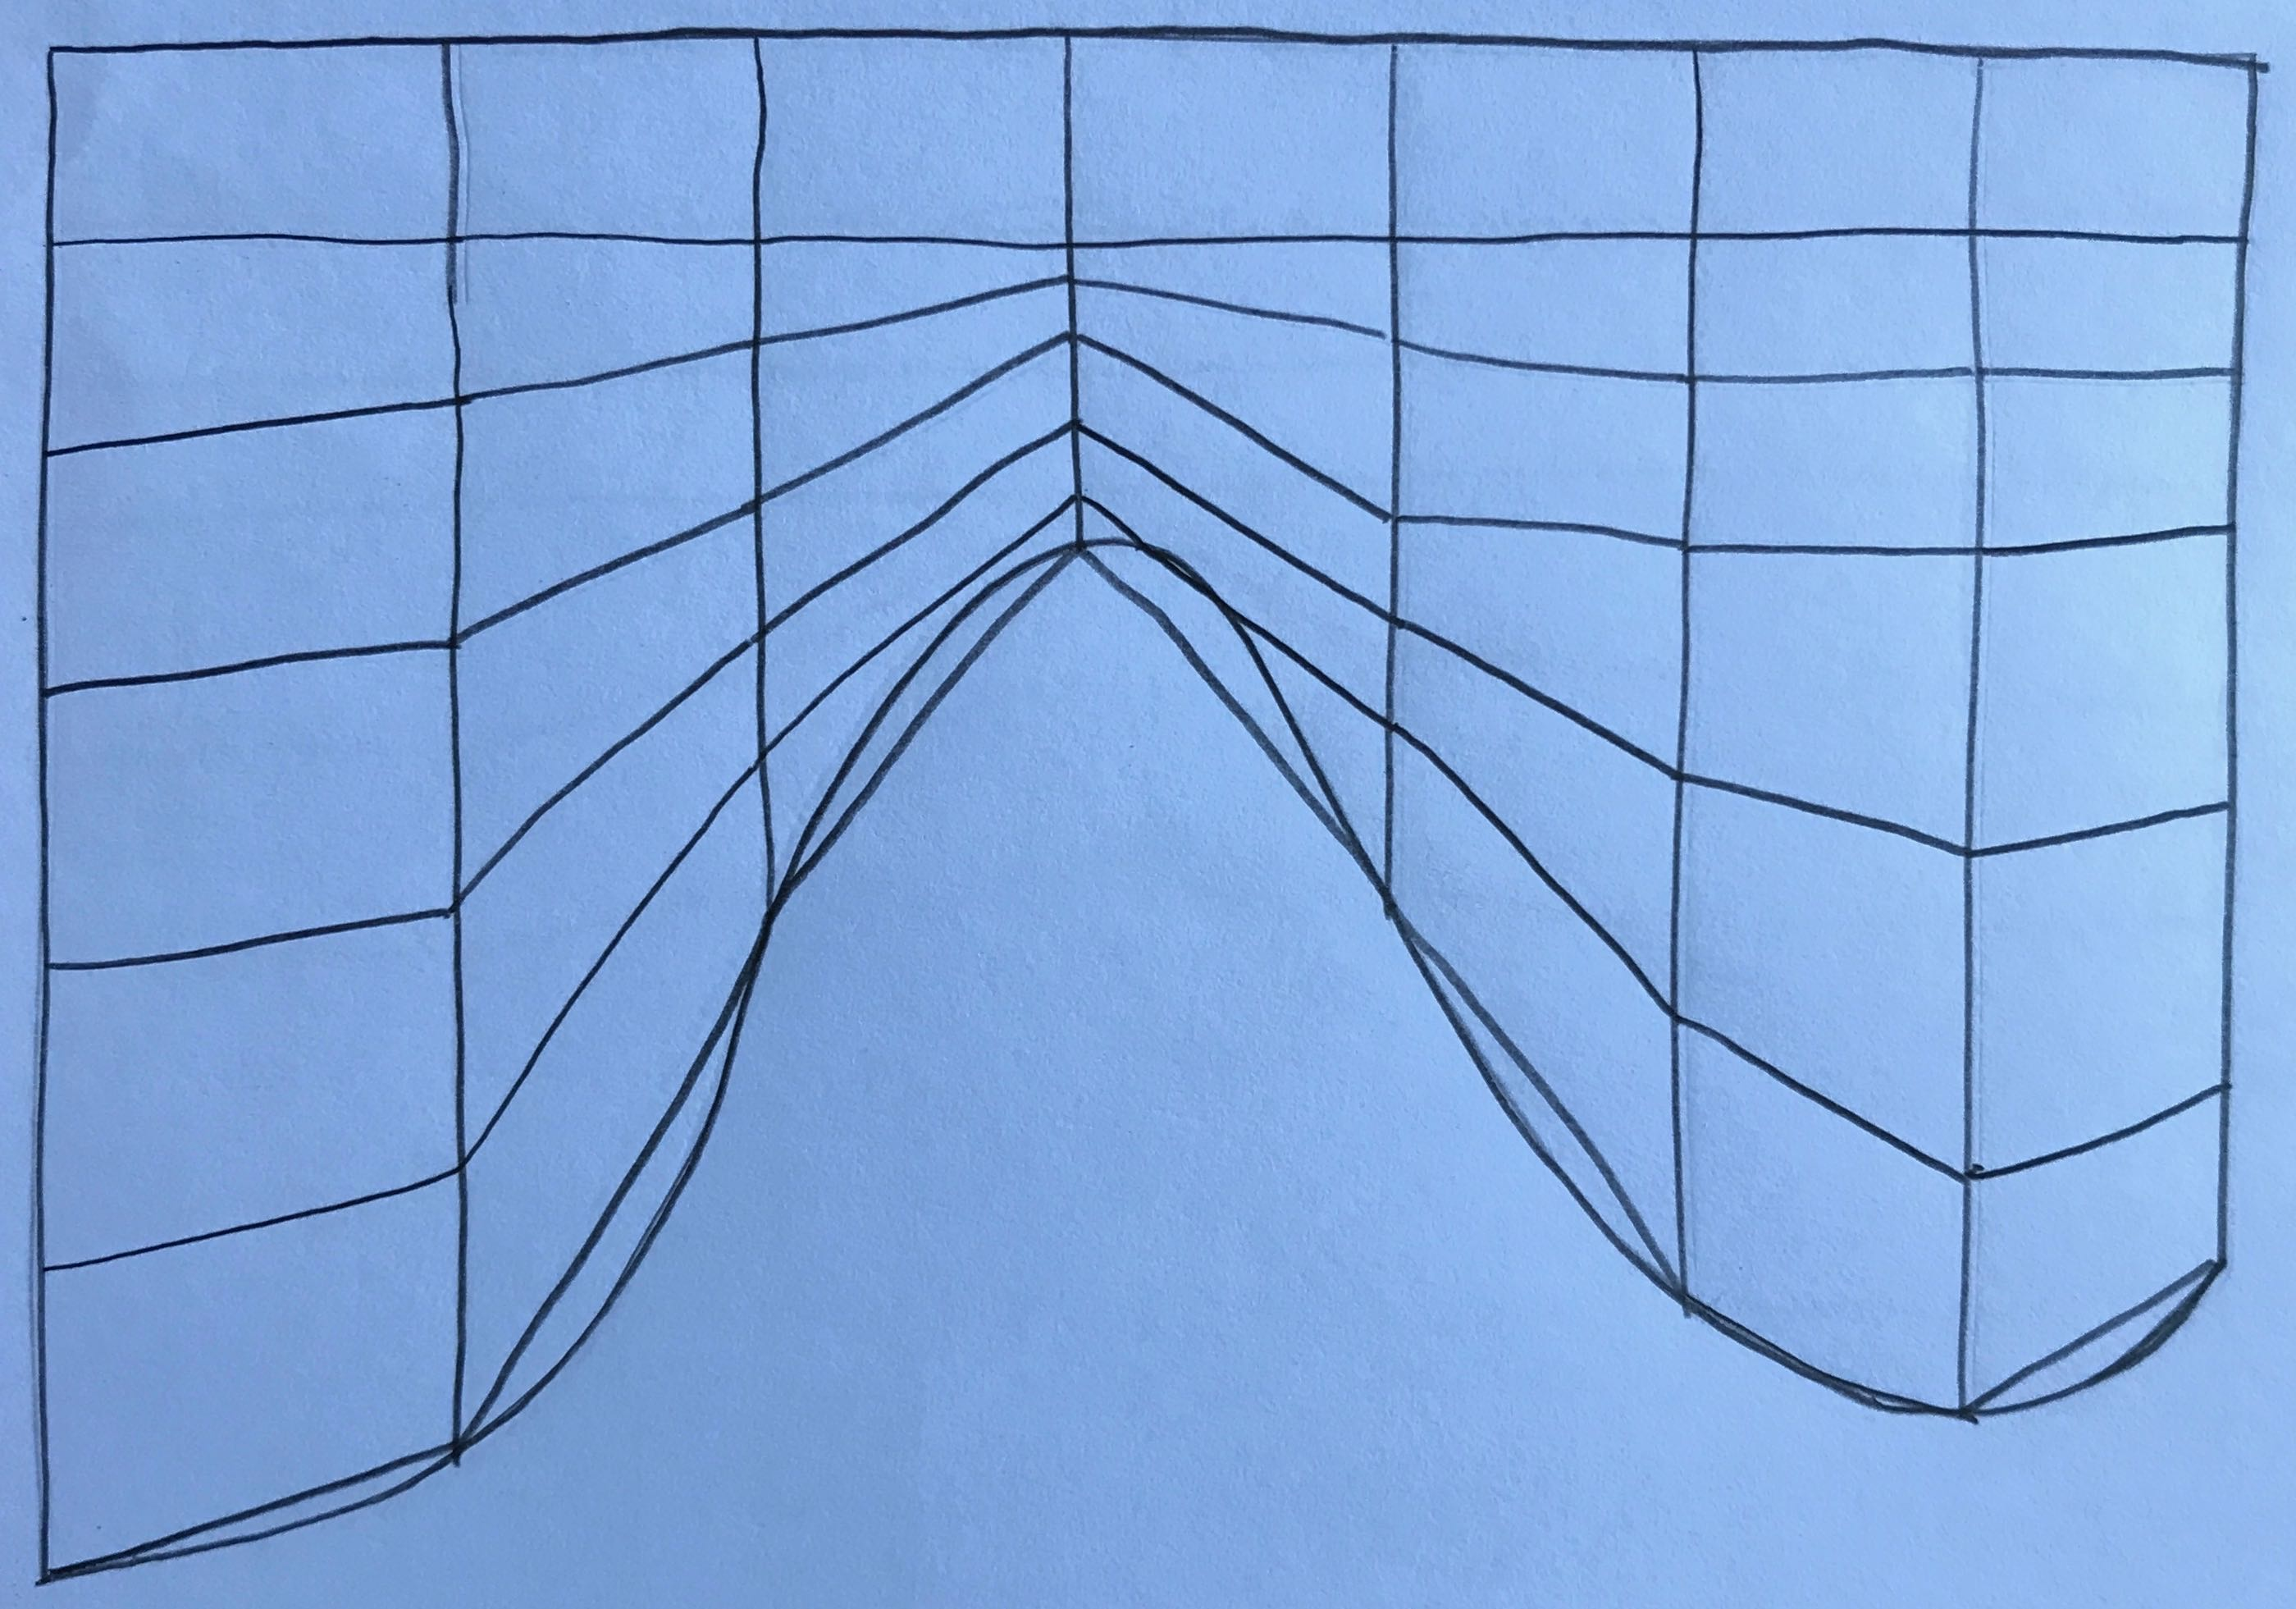
\includegraphics[width=\textwidth]{mountain-sigma}}
      \only<2>{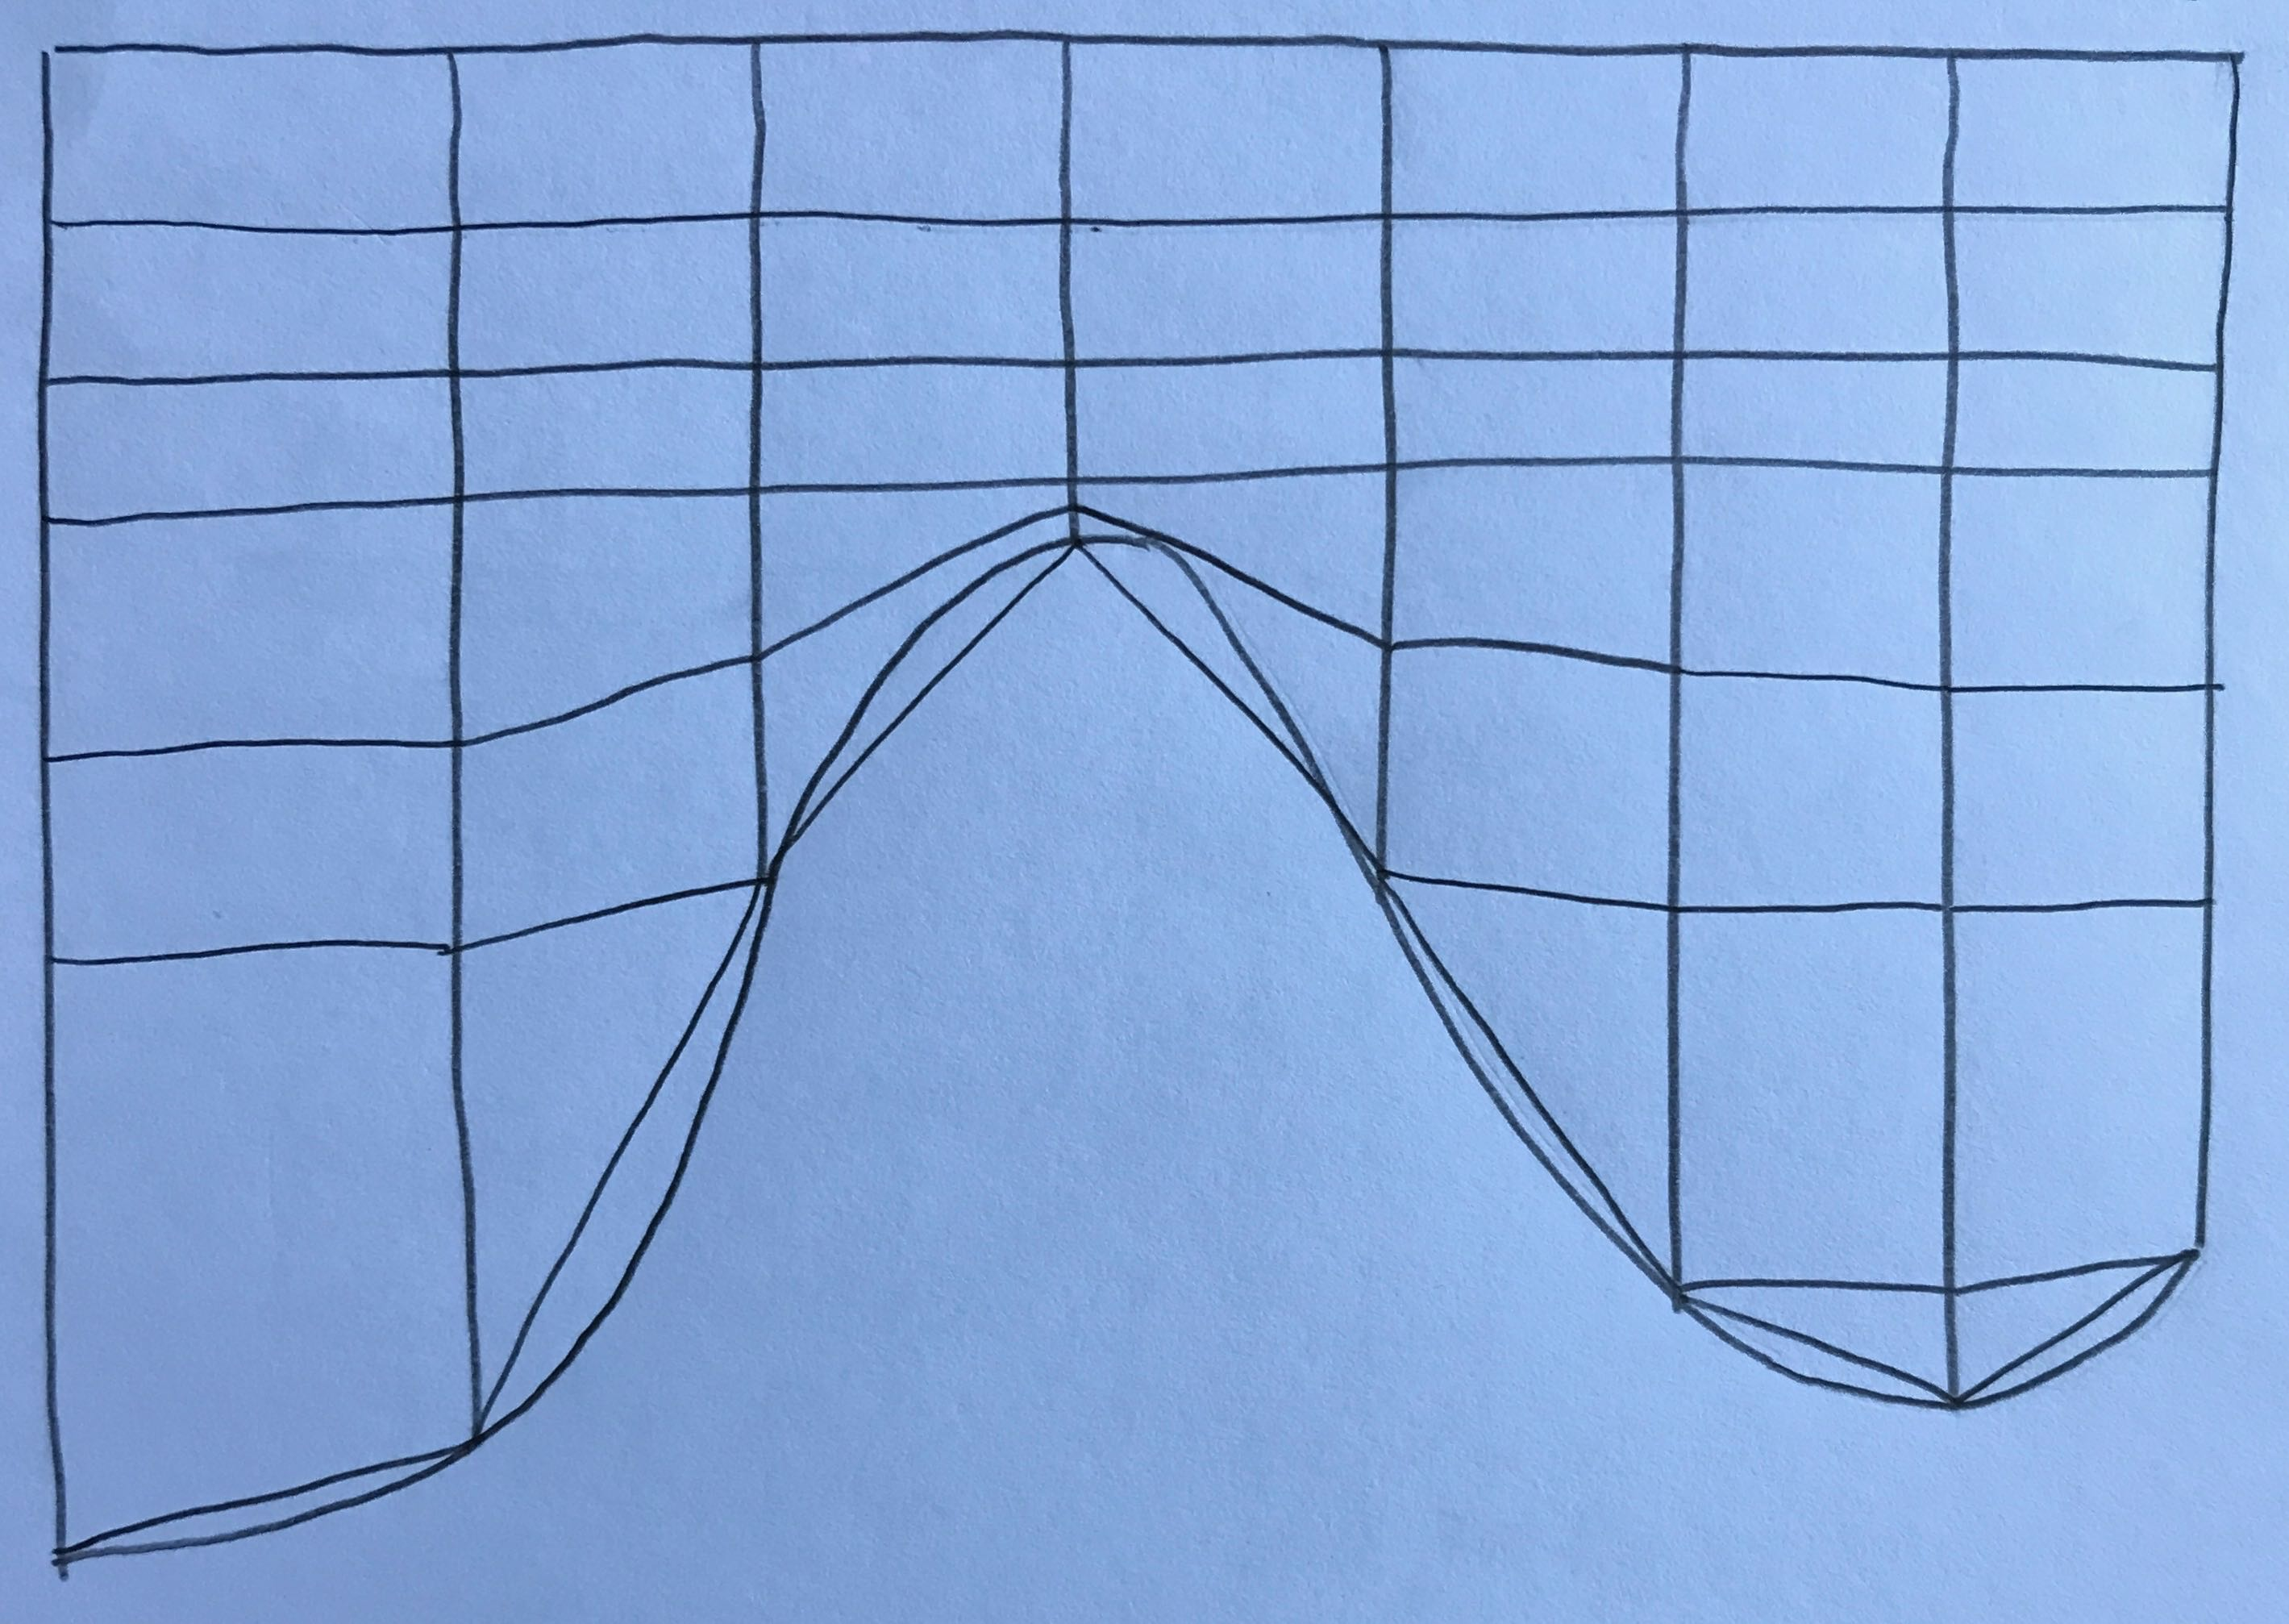
\includegraphics[width=\textwidth]{mountain-z}}
    \end{column}
  \end{columns}
\end{frame}

\begin{frame}
  \frametitle{z-layers}

  \begin{itemize}
  \item Around steep topography, might want to use z-layers rather
    than $\sigma$ coordinates.

  \item Mostly the core computational aspects remain unchanged.

  \item But, the layer number is now \emph{entity}-dependent.

  \item So there's loads more book-keeping.
  \end{itemize}
\end{frame}

\begin{frame}[plain]
  \begin{columns}
    \begin{column}{\textwidth}
      \only<1>{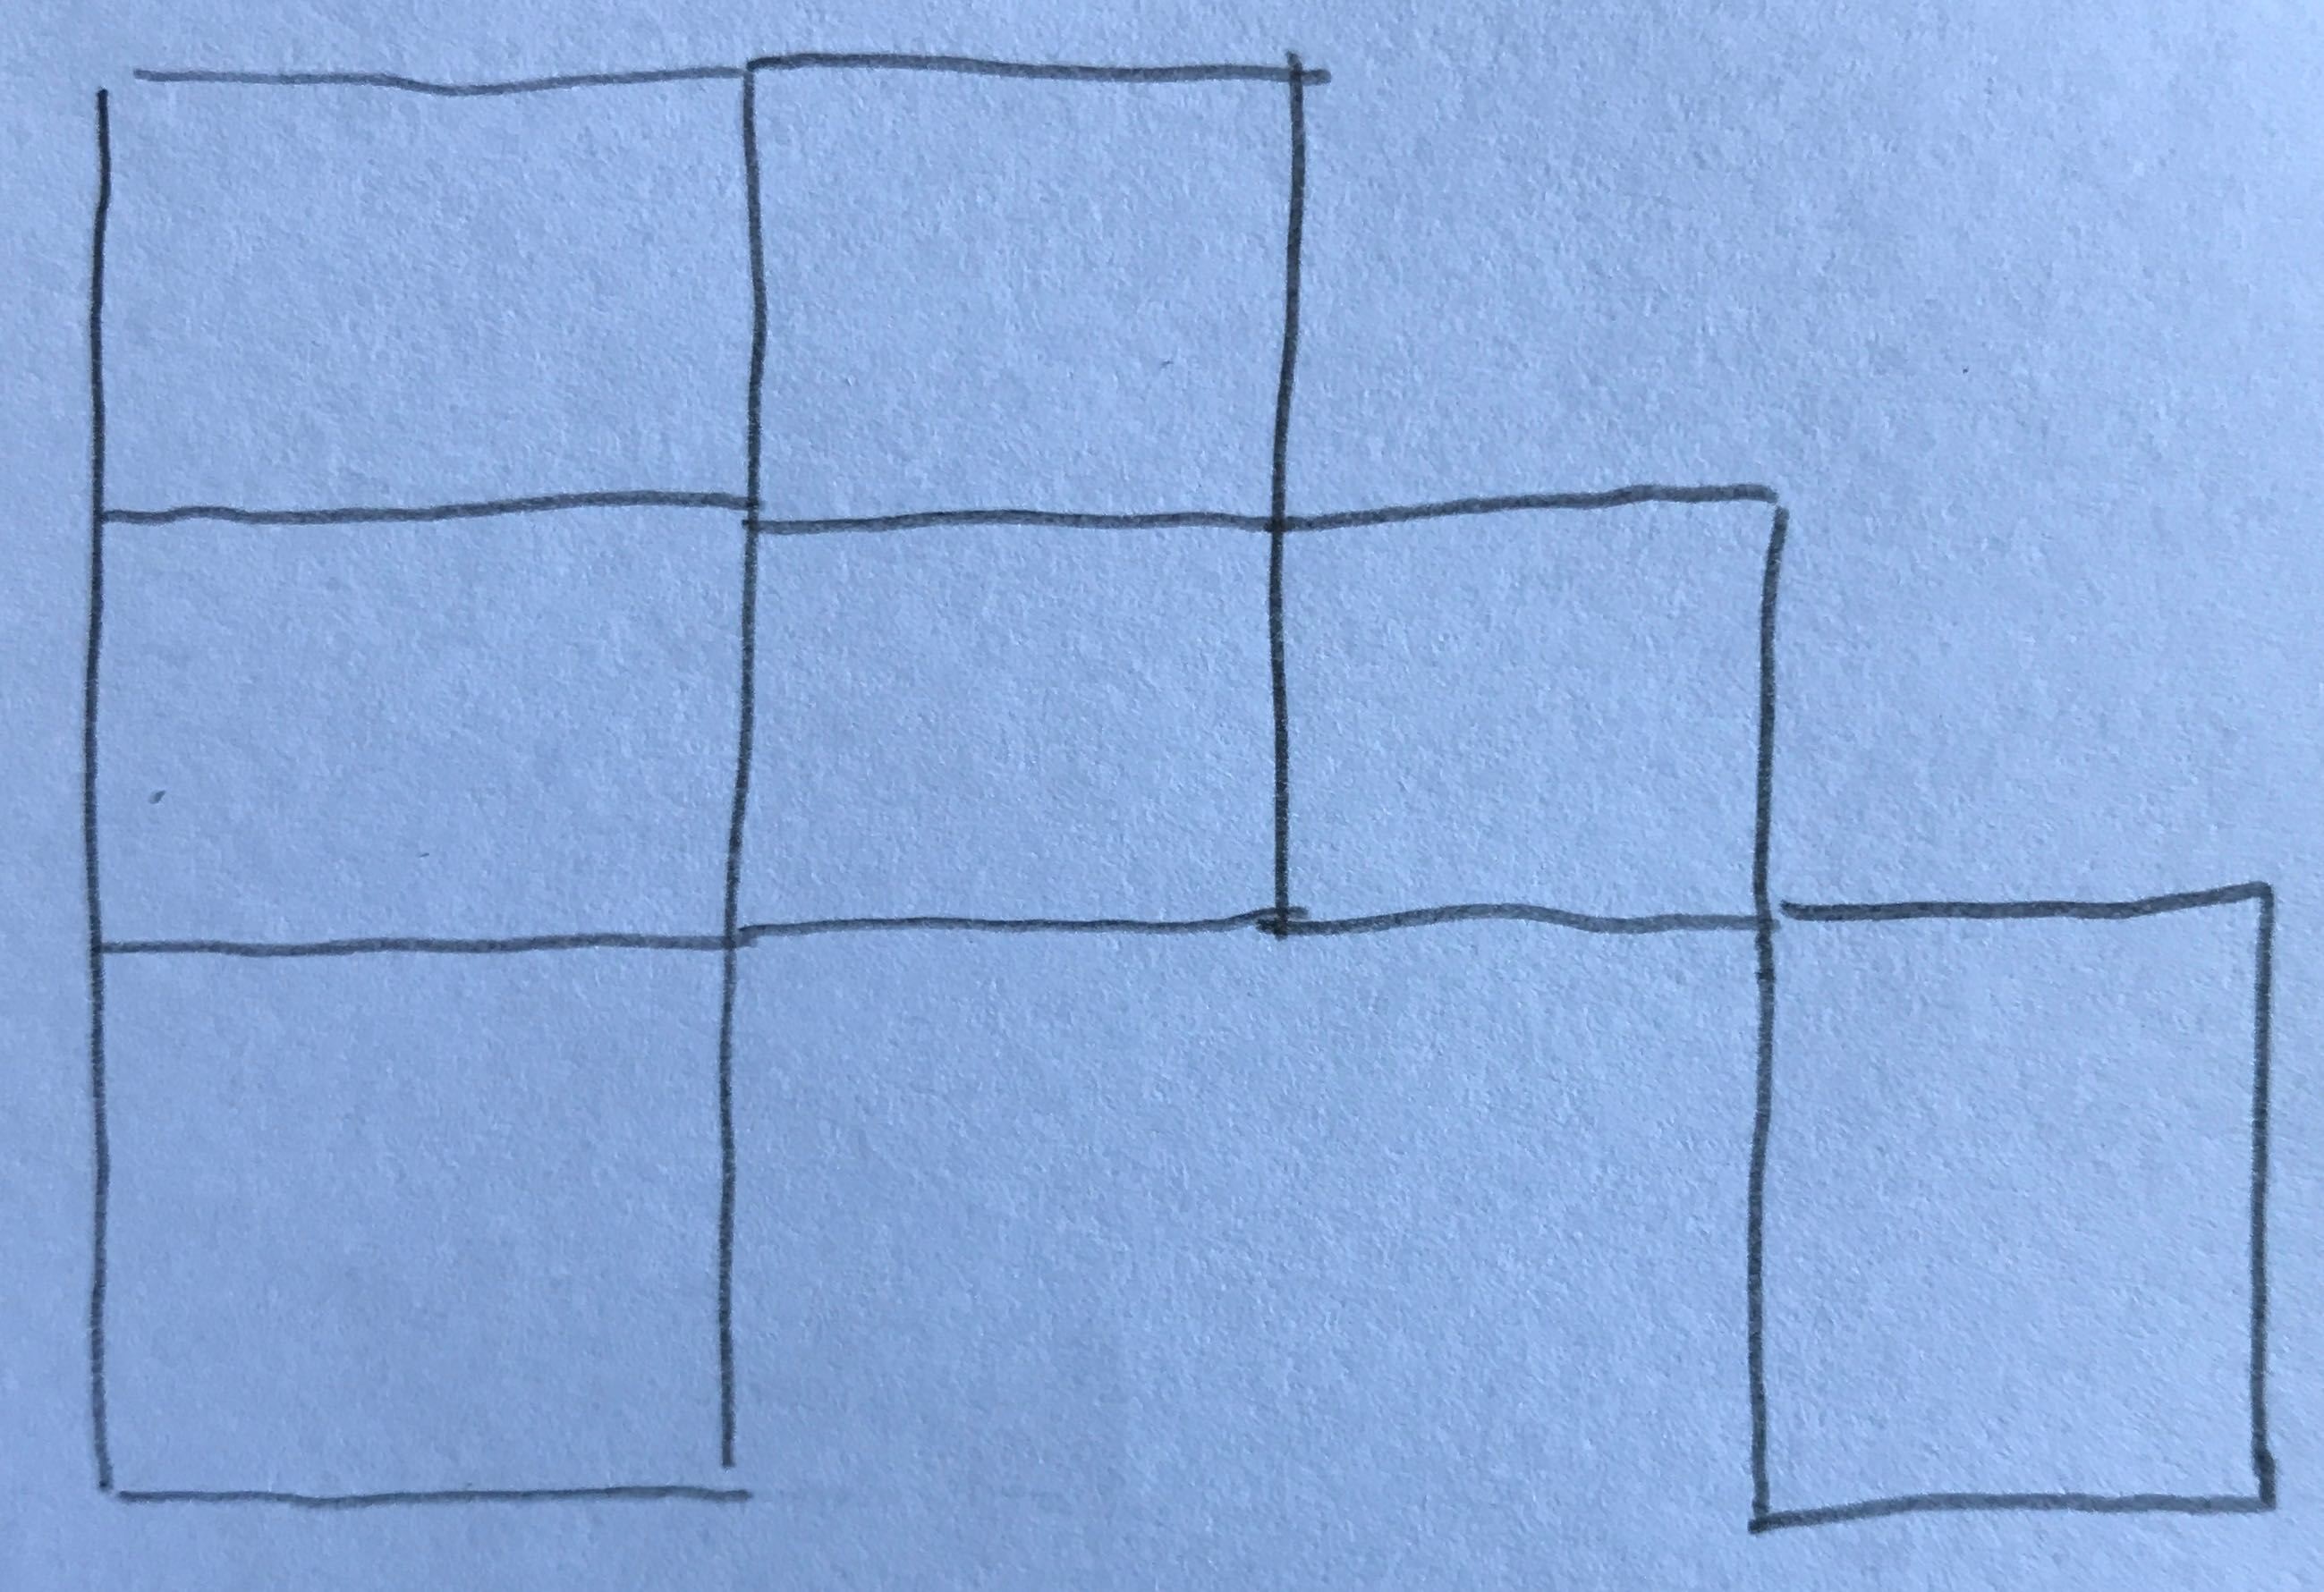
\includegraphics[width=\textwidth]{topology-2d}}
      \only<2>{Provide number of cell layers per base cell}
      \only<3>{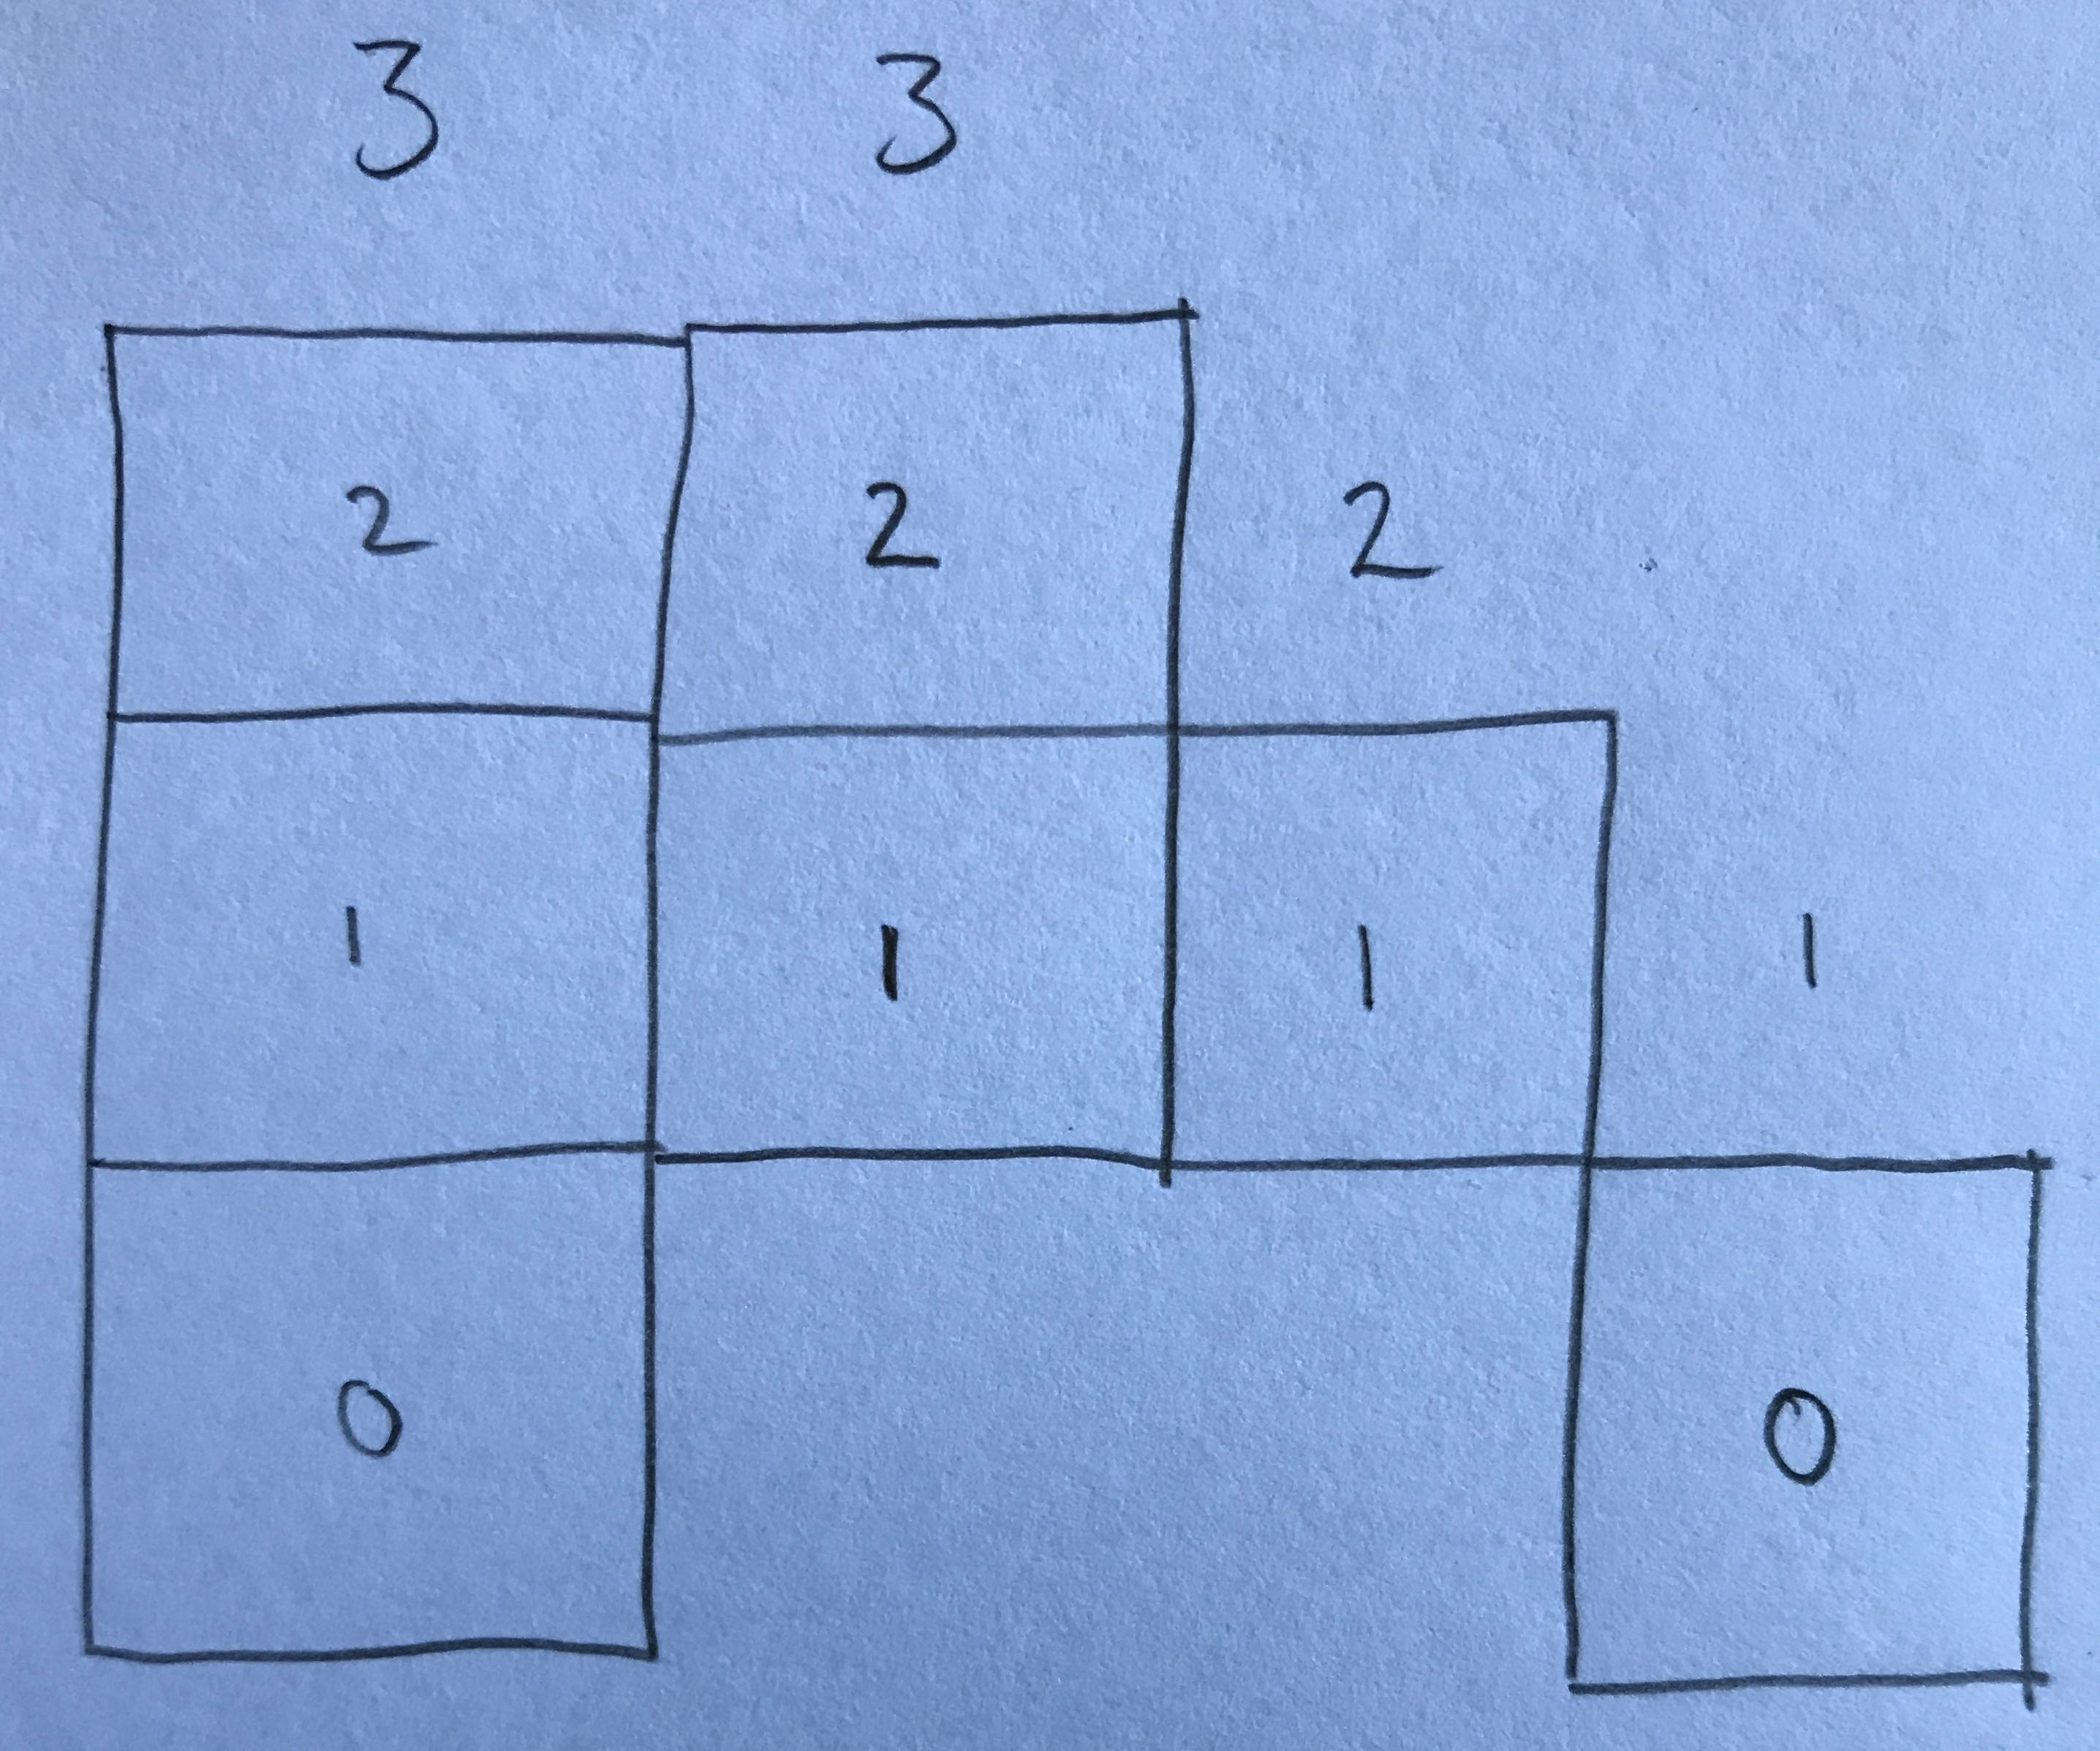
\includegraphics[width=\textwidth]{topology-2d-cells}}
      \only<4>{Bootstrap layers for other entities}
      \only<5>{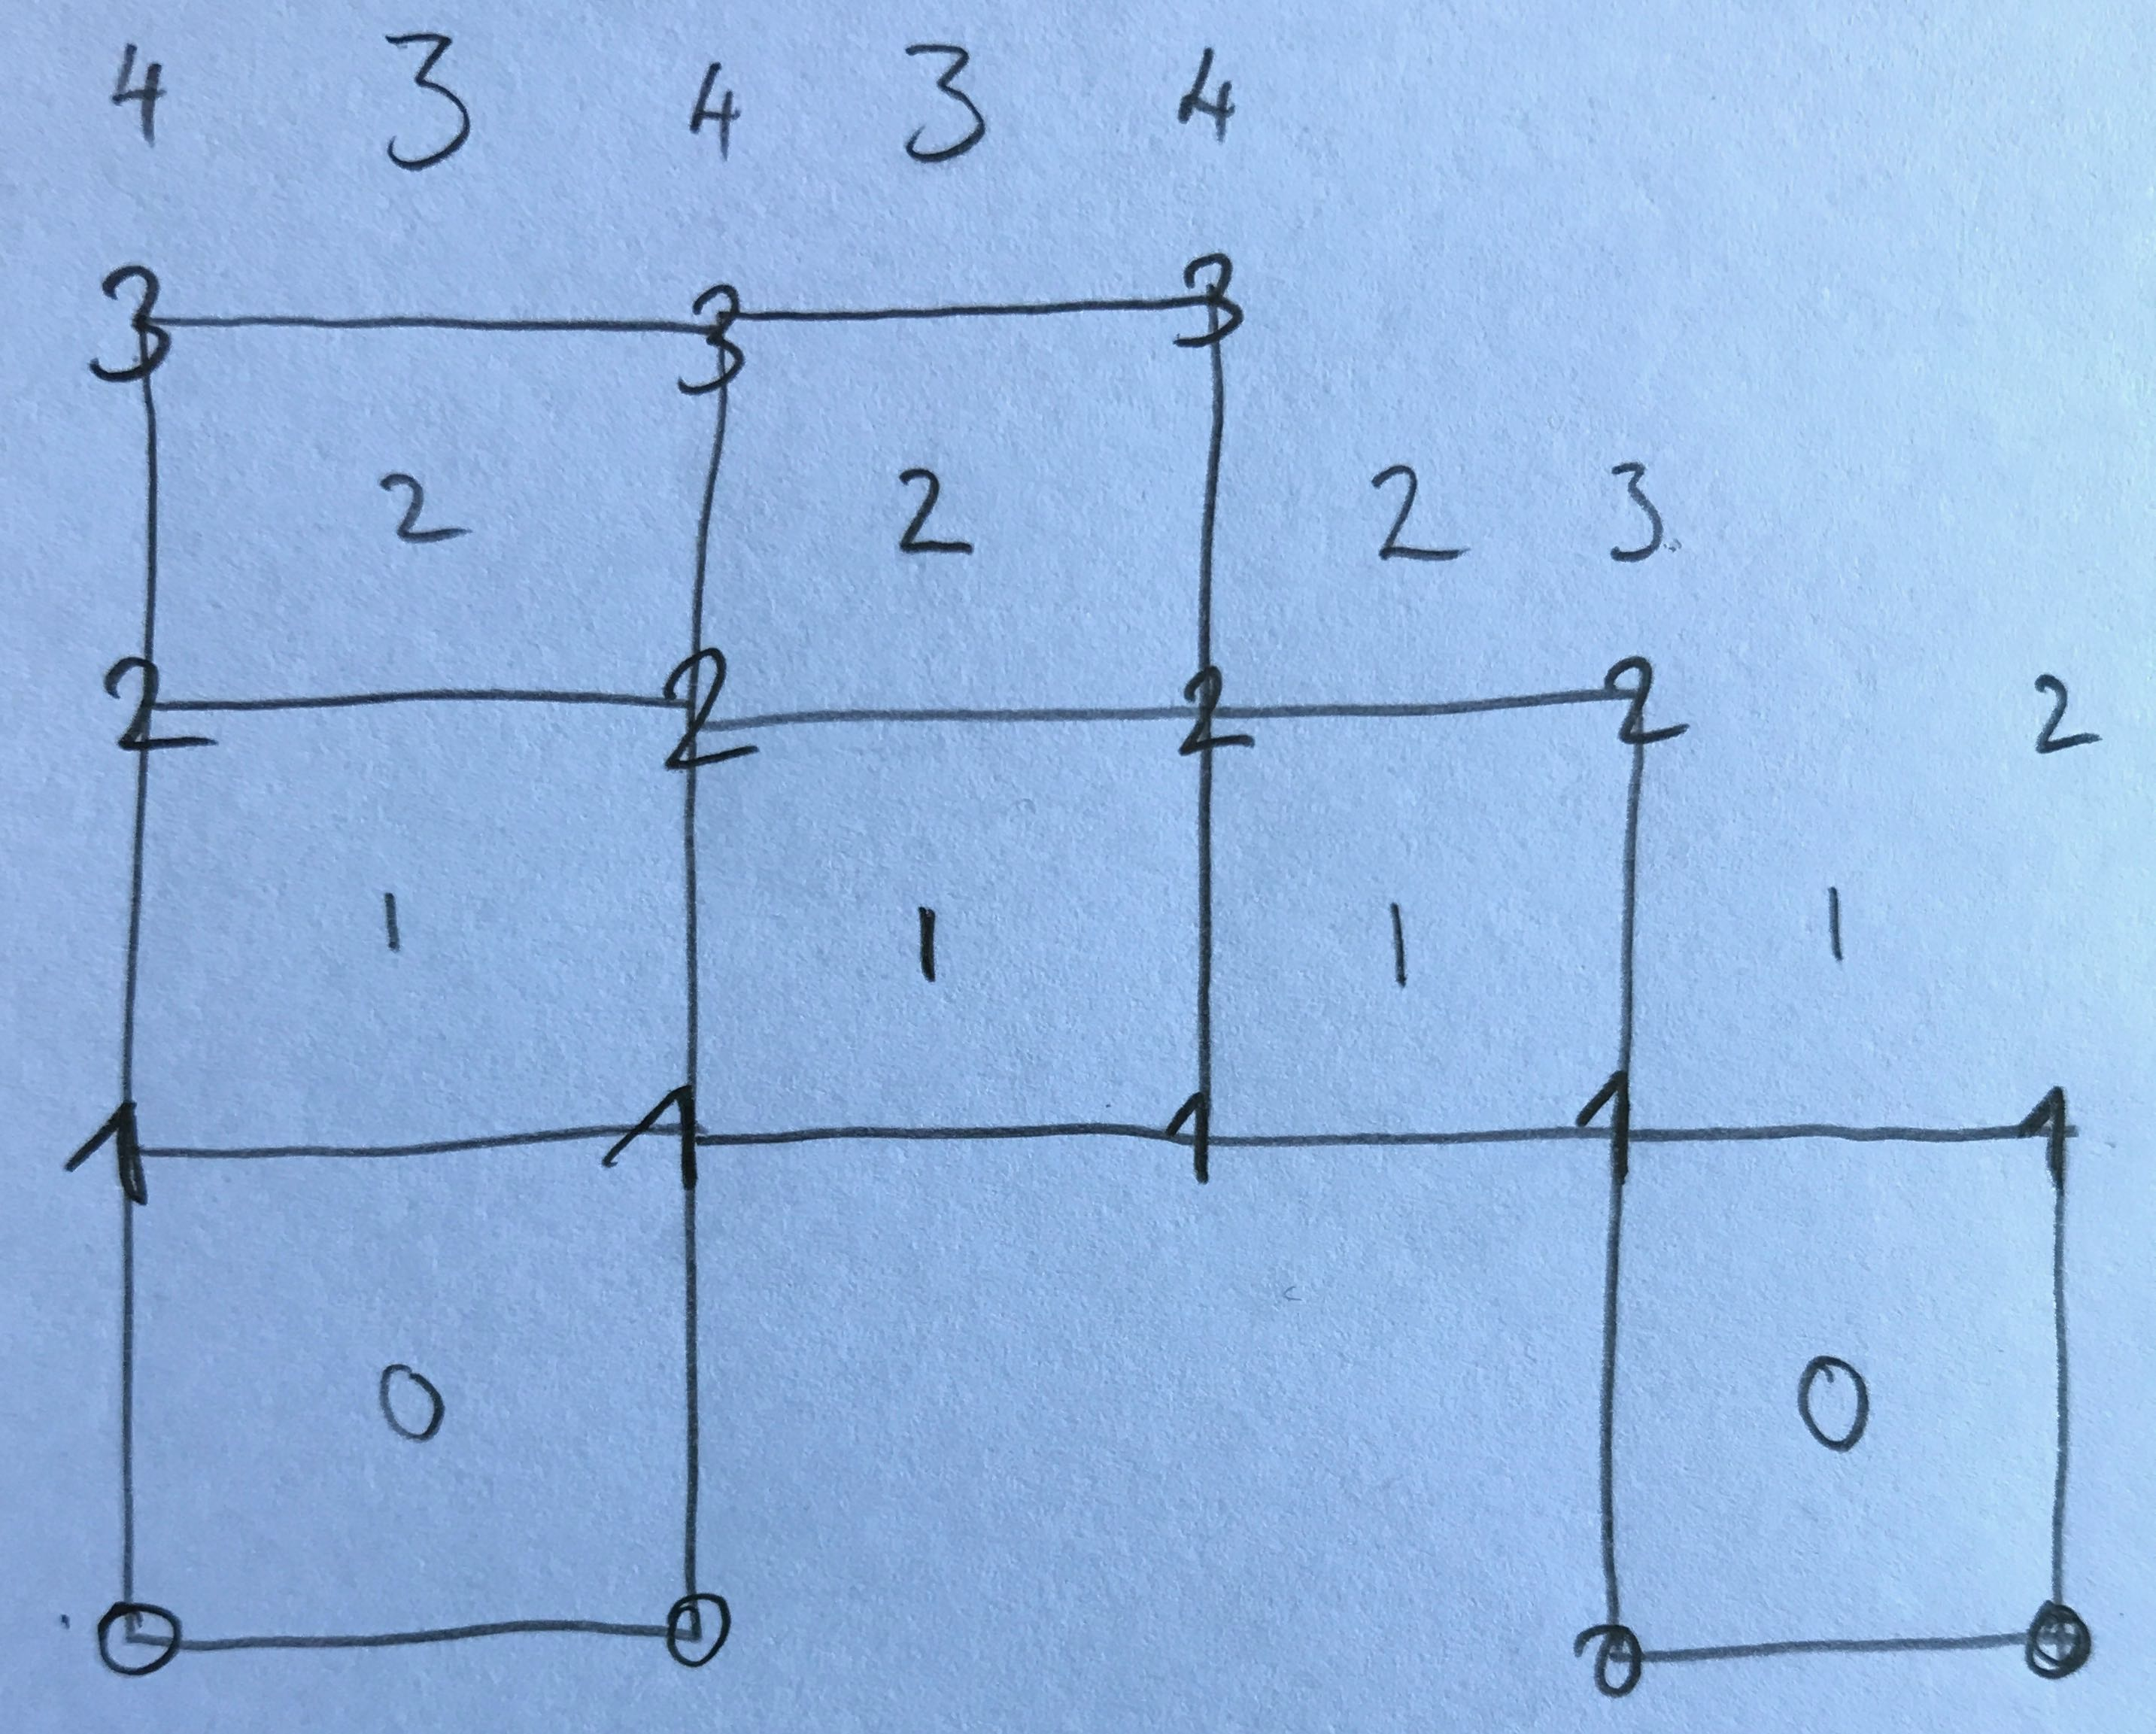
\includegraphics[width=\textwidth]{topology-2d-vertices}}
      \only<6>{Similar for 3d, but it's harder to draw}
      \only<7>{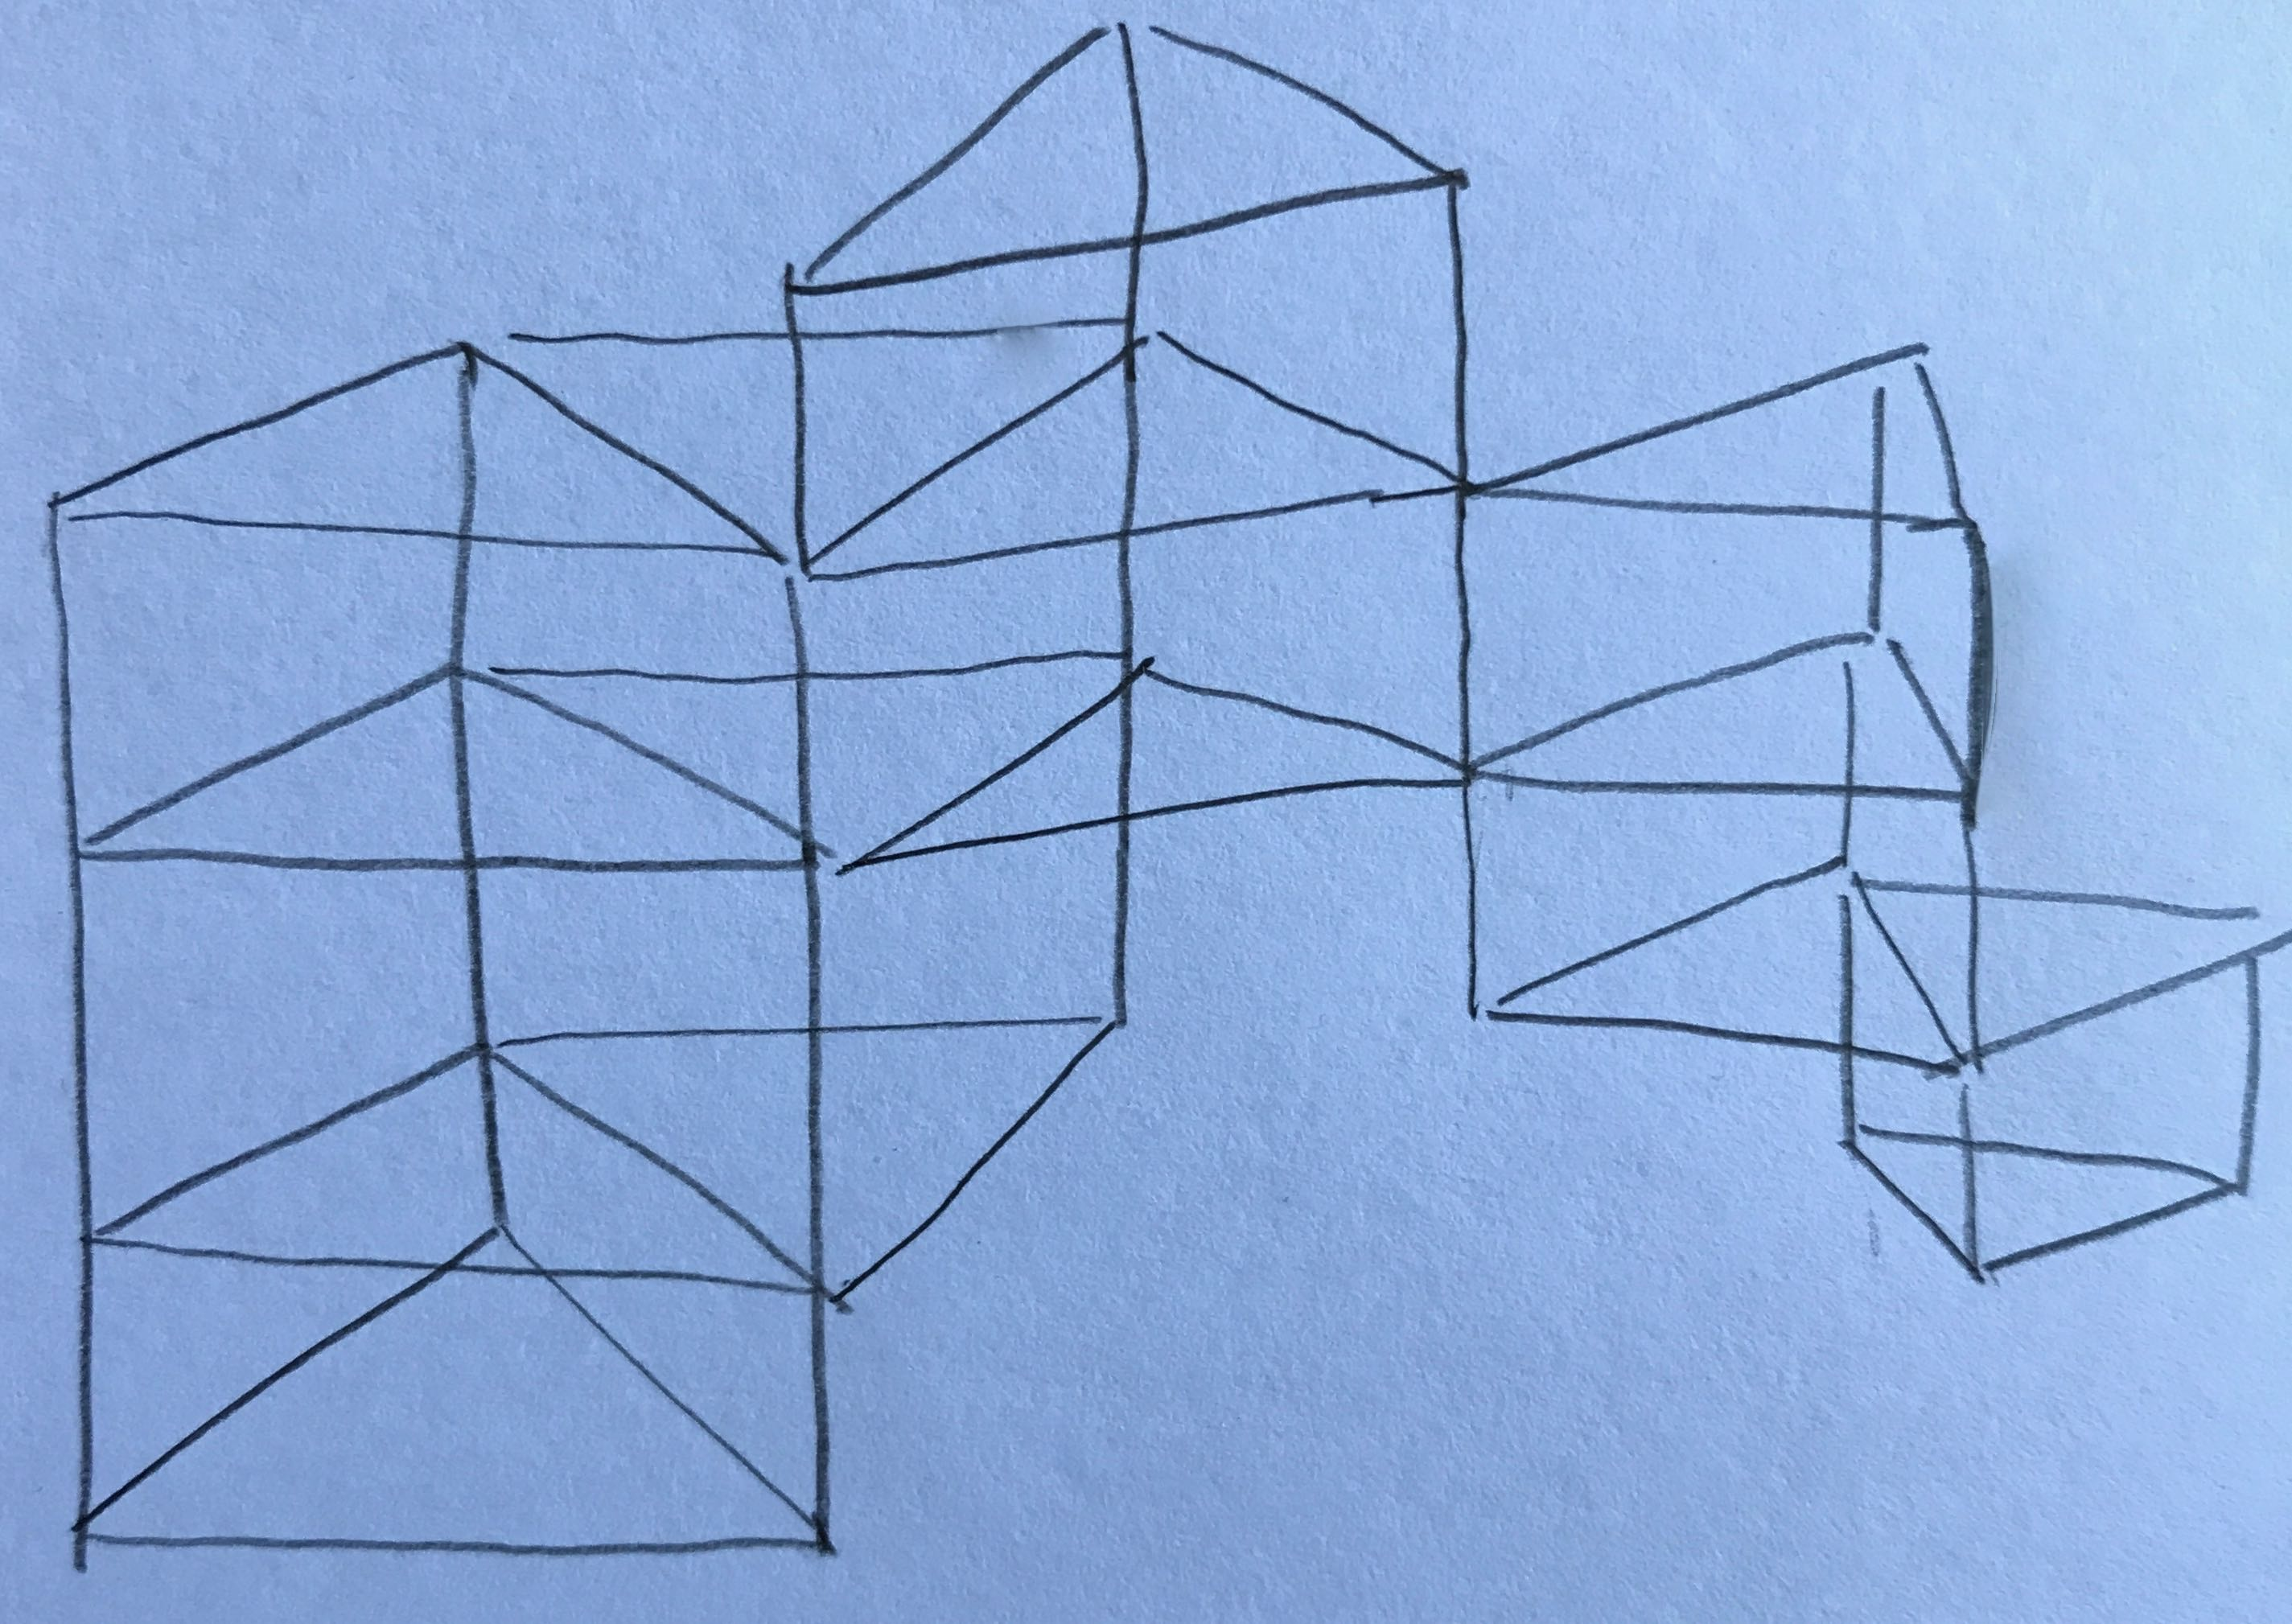
\includegraphics[width=\textwidth]{topology-3d}}
    \end{column}
  \end{columns}
\end{frame}

\begin{frame}[fragile]
  \frametitle{Datatype extension}
  Iteration sets need \emph{four} values per entry.

  \begin{overlayarea}{\textwidth}{0.7\textheight}
    \begin{onlyenv}<1>
      \begin{center}
        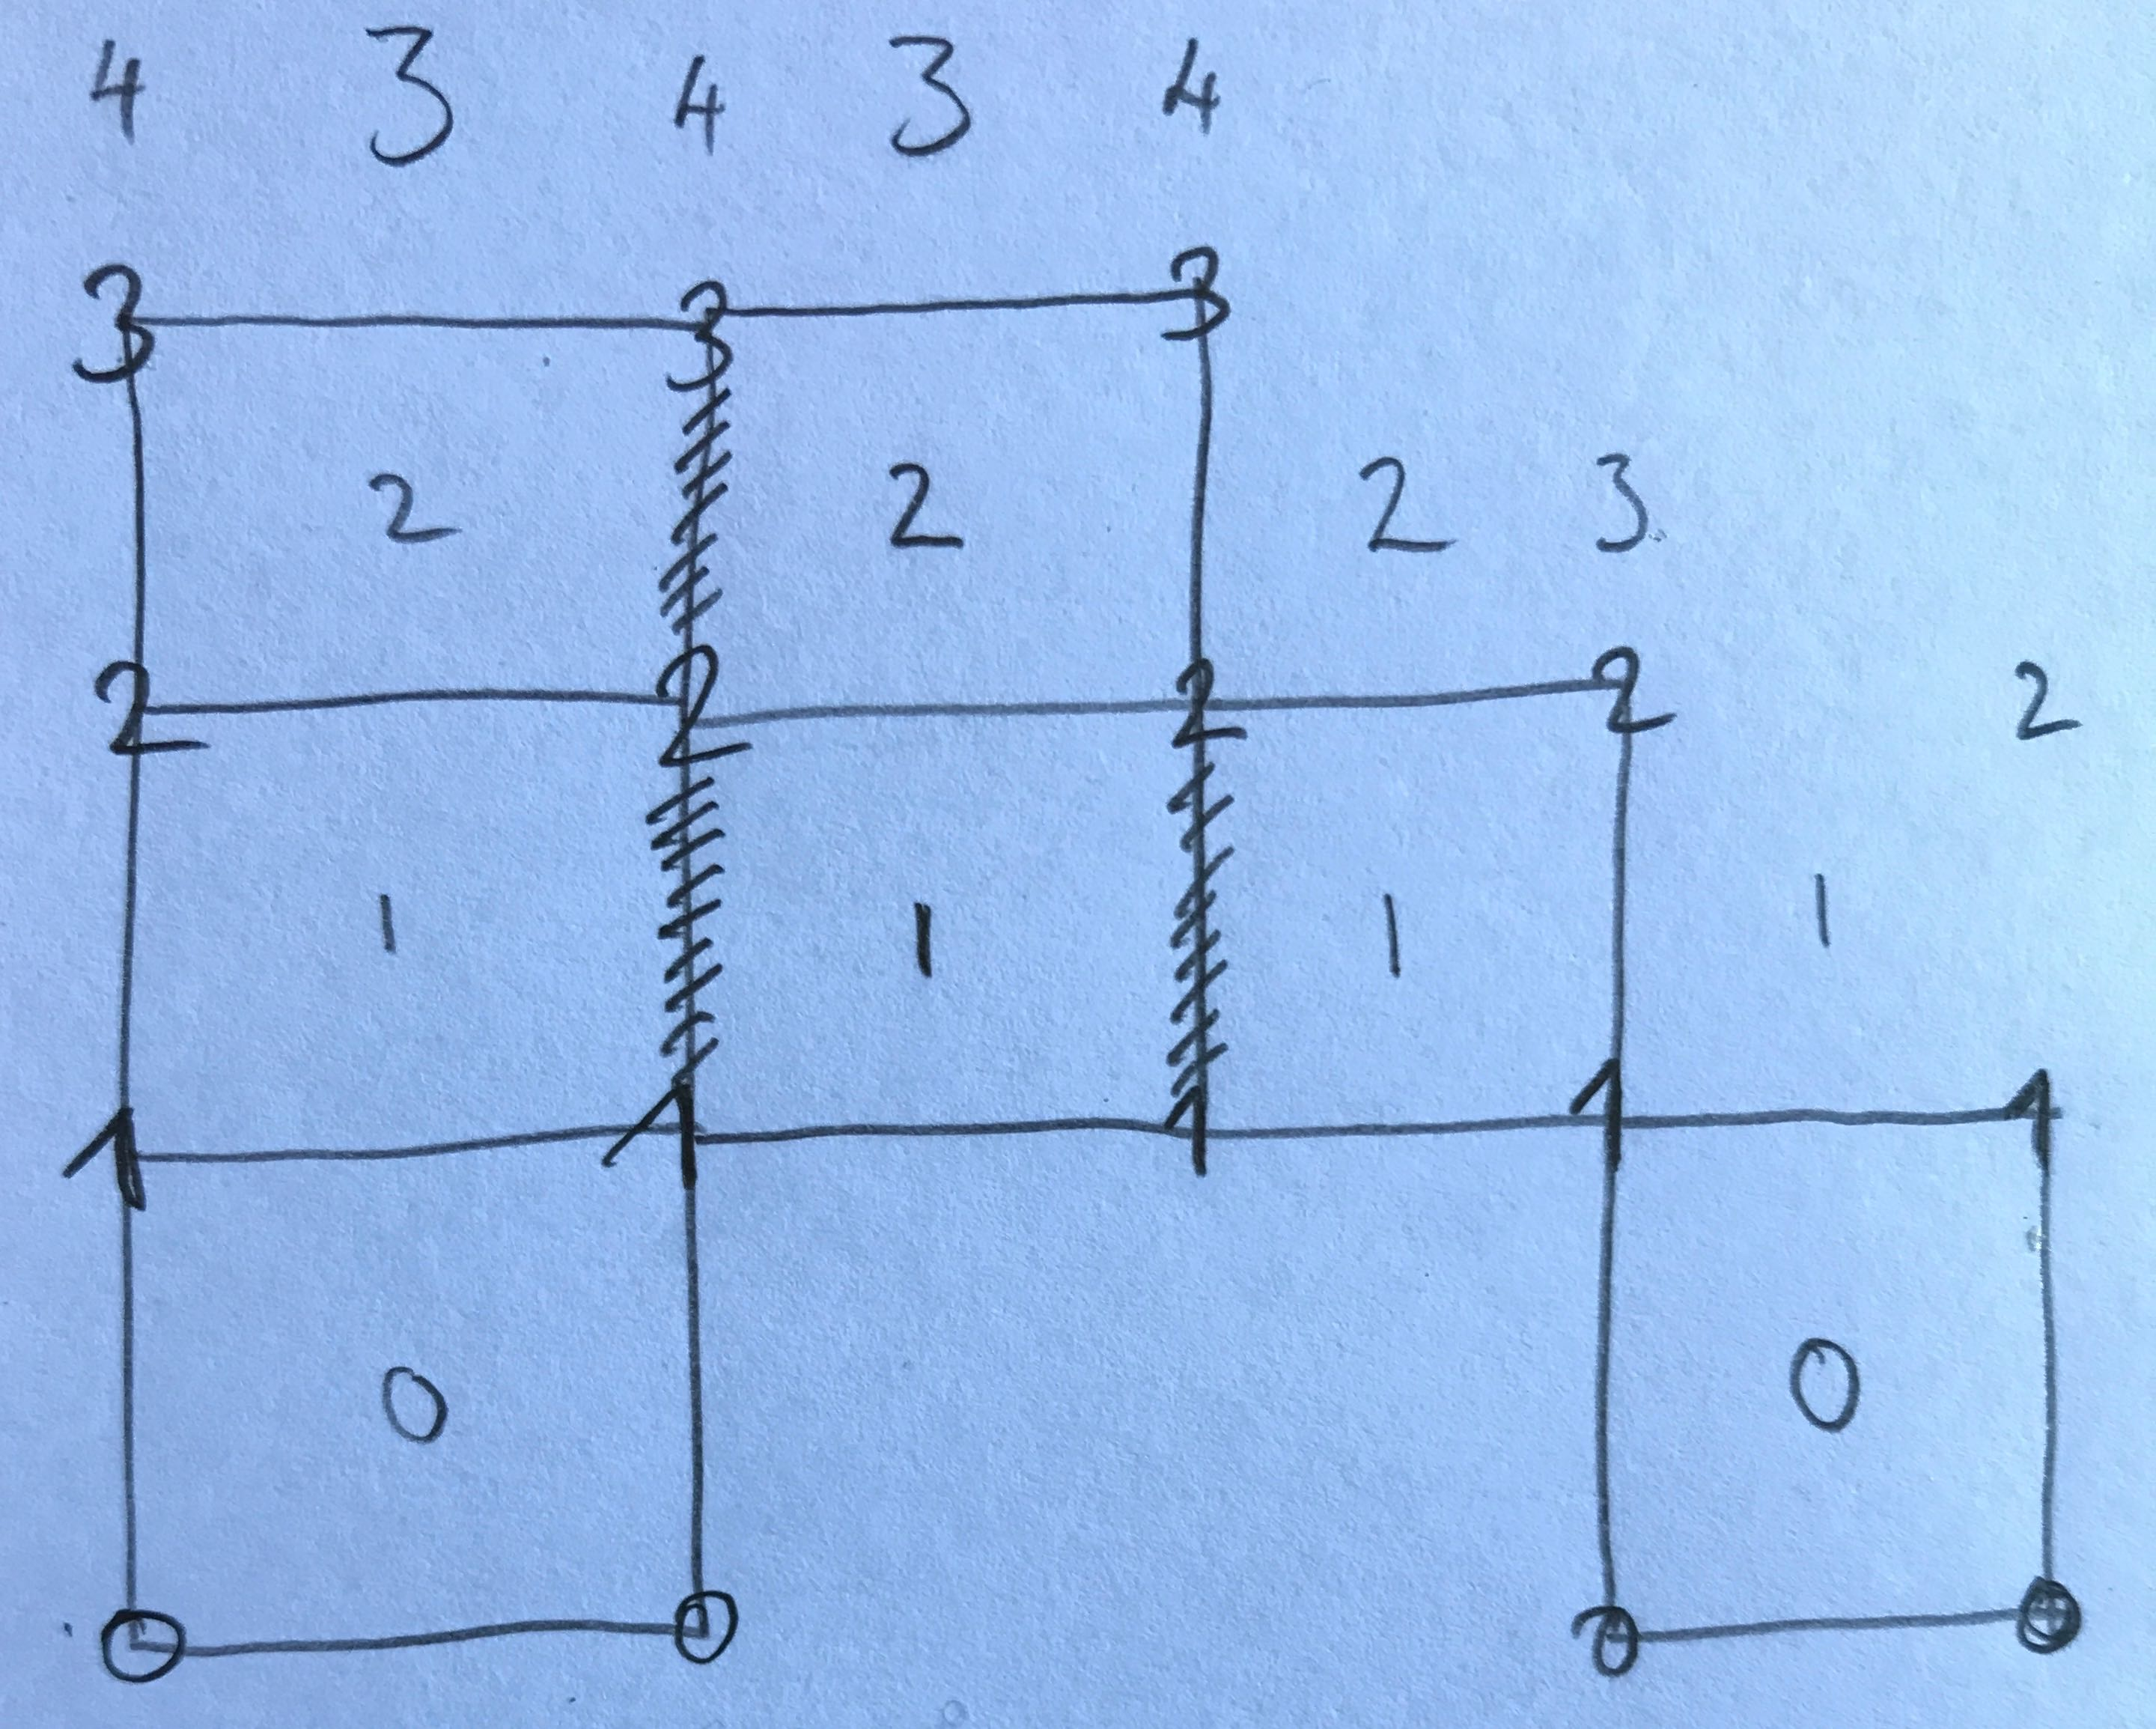
\includegraphics[height=0.7\textheight]{topology-2d-facets}
      \end{center}
    \end{onlyenv}
    \begin{onlyenv}<2>
\begin{minted}[fontsize=\scriptsize]{python}
cells = ExtrudedSet(4, layers=[[0, 3, 0, 3], 
                               [1, 3, 1, 3],
                               [1, 2, 1, 2],
                               [0, 1, 0, 1]])
efacets = ExtrudedSet(2, layers=[[0, 3, 0, 3],
                                 [0, 1, 0, 1]])
ifacets = ExtrudedSet(2, layers=[[0, 3, 1, 3],
                                 [1, 3, 1, 2]])
\end{minted}
    \end{onlyenv}
    \begin{onlyenv}<3>
      \begin{itemize}
      \item \textbf{allocation} First two entries control allocation of dofs.

        When assigning dofs to base mesh entities, we must consider
        full column.
      \item \textbf{iteration} Second two control iteration.

        When iterating over entities, we can't iterate over ``exposed''
        interior facets.
      \end{itemize}
    \end{onlyenv}
  \end{overlayarea}
\end{frame}

\begin{frame}[fragile]
  \frametitle{Kernel extension}
  \begin{itemize}
  \item GungHo \emph{kernel} encodes iteration over layers
  \item So now we need to provide this information at runtime
  \item This is just a directly accessed data array
  \item This needs to be part of kernel API.
  \end{itemize}
  \begin{overlayarea}{\textwidth}{0.5\textheight}
    \begin{onlyenv}<1>
\begin{minted}[fontsize=\tiny]{fortran}
subroutine old_kernel(A, B, nlayers)
   ...
   integer, intent(in) :: nlayers

   do k = 0, nlayers-1
    ...
   end do
end subroutine old_kernel
\end{minted}
    \end{onlyenv}    
    \begin{onlyenv}<2>
\begin{minted}[fontsize=\tiny]{fortran}
subroutine new_kernel(A, B, layer_begin, layer_end)
   ...
   integer, intent(in) :: layer_begin, layer_end

   do k = layer_begin, layer_end
    ...
   end do
end subroutine new_kernel
\end{minted}
    \end{onlyenv}
  \end{overlayarea}
\end{frame}
\begin{frame}
  \frametitle{Firedrake support}
  \begin{itemize}
  \item Support is still WIP (interior facets)
  \item We squash interior facets geometrically, but not
    topologically.
  \item Then we never iterate over these facets.
  \item They could be left exposed, but now need new iteration type.
  \item An alternate option would be mixed cell shape (ugh!)
  \end{itemize}
\end{frame}
\end{document}
